% Options for packages loaded elsewhere
\PassOptionsToPackage{unicode}{hyperref}
\PassOptionsToPackage{hyphens}{url}
%
\documentclass[
]{article}
\title{Analysis of the Global Extreme Poverty}
\author{Group16}
\date{2022/2/16}

\usepackage{amsmath,amssymb}
\usepackage{lmodern}
\usepackage{iftex}
\ifPDFTeX
  \usepackage[T1]{fontenc}
  \usepackage[utf8]{inputenc}
  \usepackage{textcomp} % provide euro and other symbols
\else % if luatex or xetex
  \usepackage{unicode-math}
  \defaultfontfeatures{Scale=MatchLowercase}
  \defaultfontfeatures[\rmfamily]{Ligatures=TeX,Scale=1}
\fi
% Use upquote if available, for straight quotes in verbatim environments
\IfFileExists{upquote.sty}{\usepackage{upquote}}{}
\IfFileExists{microtype.sty}{% use microtype if available
  \usepackage[]{microtype}
  \UseMicrotypeSet[protrusion]{basicmath} % disable protrusion for tt fonts
}{}
\makeatletter
\@ifundefined{KOMAClassName}{% if non-KOMA class
  \IfFileExists{parskip.sty}{%
    \usepackage{parskip}
  }{% else
    \setlength{\parindent}{0pt}
    \setlength{\parskip}{6pt plus 2pt minus 1pt}}
}{% if KOMA class
  \KOMAoptions{parskip=half}}
\makeatother
\usepackage{xcolor}
\IfFileExists{xurl.sty}{\usepackage{xurl}}{} % add URL line breaks if available
\IfFileExists{bookmark.sty}{\usepackage{bookmark}}{\usepackage{hyperref}}
\hypersetup{
  pdftitle={Analysis of the Global Extreme Poverty},
  pdfauthor={Group16},
  hidelinks,
  pdfcreator={LaTeX via pandoc}}
\urlstyle{same} % disable monospaced font for URLs
\usepackage[margin=1in]{geometry}
\usepackage{longtable,booktabs,array}
\usepackage{calc} % for calculating minipage widths
% Correct order of tables after \paragraph or \subparagraph
\usepackage{etoolbox}
\makeatletter
\patchcmd\longtable{\par}{\if@noskipsec\mbox{}\fi\par}{}{}
\makeatother
% Allow footnotes in longtable head/foot
\IfFileExists{footnotehyper.sty}{\usepackage{footnotehyper}}{\usepackage{footnote}}
\makesavenoteenv{longtable}
\usepackage{graphicx}
\makeatletter
\def\maxwidth{\ifdim\Gin@nat@width>\linewidth\linewidth\else\Gin@nat@width\fi}
\def\maxheight{\ifdim\Gin@nat@height>\textheight\textheight\else\Gin@nat@height\fi}
\makeatother
% Scale images if necessary, so that they will not overflow the page
% margins by default, and it is still possible to overwrite the defaults
% using explicit options in \includegraphics[width, height, ...]{}
\setkeys{Gin}{width=\maxwidth,height=\maxheight,keepaspectratio}
% Set default figure placement to htbp
\makeatletter
\def\fps@figure{htbp}
\makeatother
\setlength{\emergencystretch}{3em} % prevent overfull lines
\providecommand{\tightlist}{%
  \setlength{\itemsep}{0pt}\setlength{\parskip}{0pt}}
\setcounter{secnumdepth}{5}
\ifLuaTeX
  \usepackage{selnolig}  % disable illegal ligatures
\fi

\begin{document}
\maketitle

=======

\hypertarget{introduction}{%
\section{Introduction}\label{introduction}}

Most people in the world are in the poverty. This analysis is aim to
explore the global extreme poverty, which is considered a person if they
live on less than 1.90 dollars per day, defined by the United Nation. We
have used 5 data sets to analyze extreme poverty. The distribution of
population between different poverty thresholds from 1981 to 2017, total
GDP, and the total expenditure as a share of GDP for that year in health
care, education, and military. In this report, we just focus on 2012 to
2017. We will be discussing two questions: 1. What is the state of
extreme poverty in the world? And the prediction of the population of
extreme poverty. 2. How do these factors influence extreme poverty in
the world?

\hypertarget{exploratory-data-analysis}{%
\section{Exploratory Data Analysis}\label{exploratory-data-analysis}}

\hypertarget{what-is-the-state-of-extreme-poverty-in-the-world}{%
\subsection{What is the state of extreme poverty in the
world?}\label{what-is-the-state-of-extreme-poverty-in-the-world}}

As defined by the World Bank, extreme poverty is the person who living
on \$1.90 per day. From the figure 1 we can know that the government has
made great efforts to reduce the number of people living in extreme
poverty. Between 1980 and 2017, the number of people living in extreme
poverty in the world has been decreasing.

\begin{figure}[H]

{\centering 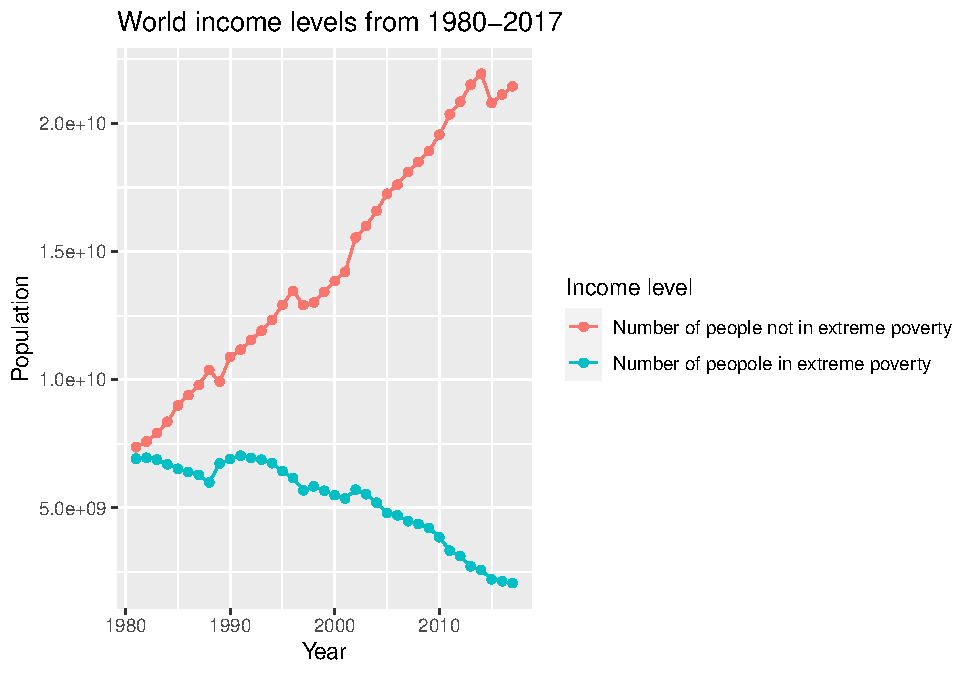
\includegraphics[width=0.68\linewidth]{Poster_Formal_files/figure-latex/table1-1} 

}

\caption{\label{fig:line} line chart of 100 employees.}\label{fig:table1}
\end{figure}

\begin{figure}[H]

{\centering 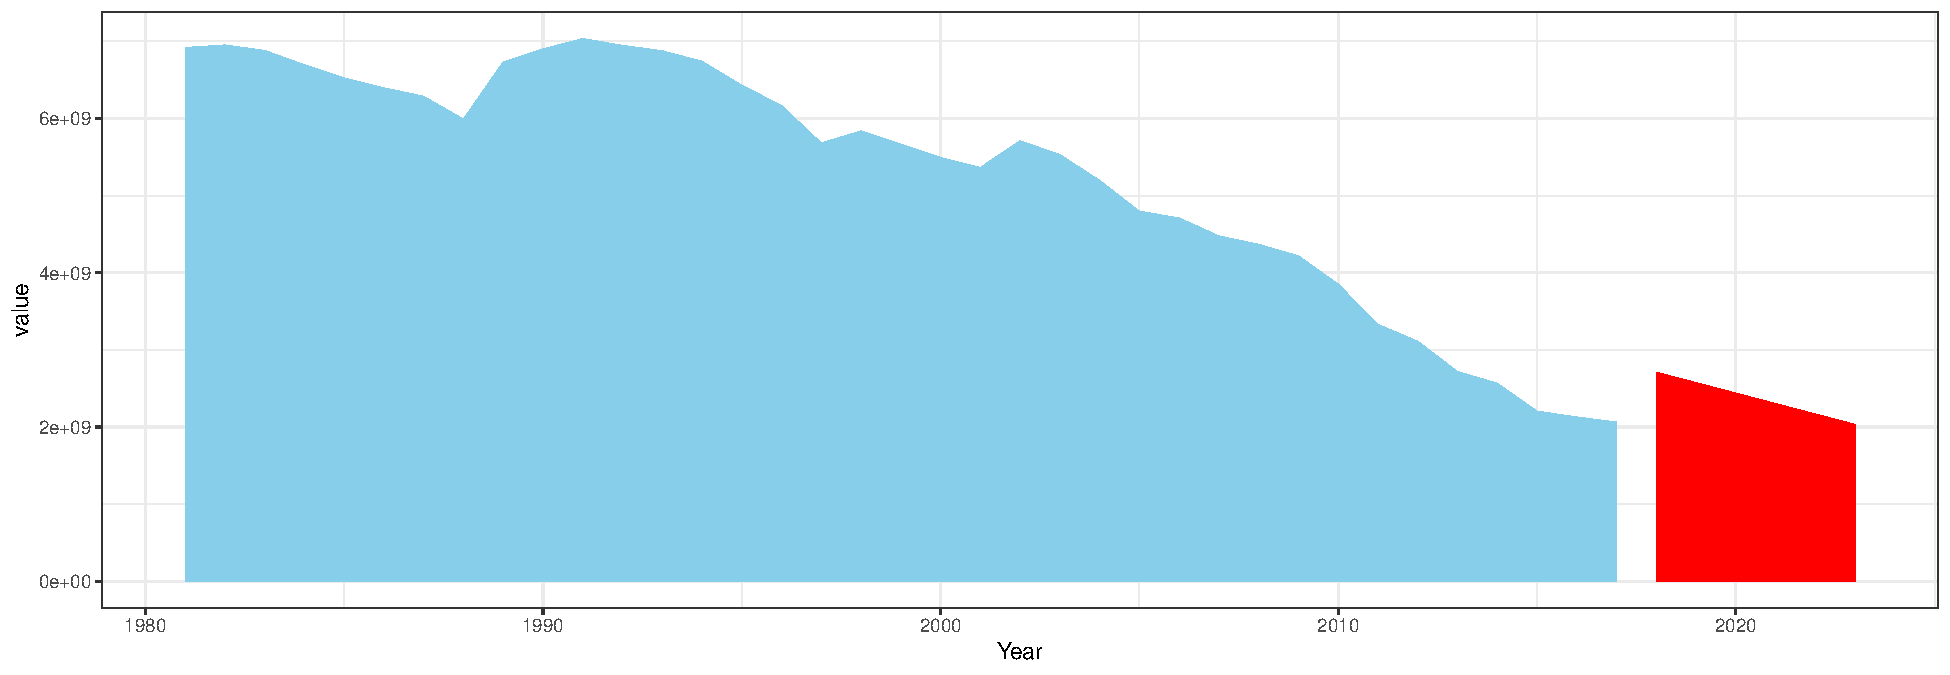
\includegraphics{Poster_Formal_files/figure-latex/creat modle-1} 

}

\caption{\label{fig:resids} Scatterplots of the residuals by working years and a histogram of the residuals (right).}\label{fig:creat modle}
\end{figure}

\begin{longtable}[]{@{}ll@{}}
\caption{Data summary}\tabularnewline
\toprule
\endhead
Name & data\_2012\_2017 \\
Number of rows & 540 \\
Number of columns & 7 \\
\_\_\_\_\_\_\_\_\_\_\_\_\_\_\_\_\_\_\_\_\_\_\_ & \\
Column type frequency: & \\
character & 2 \\
numeric & 5 \\
\_\_\_\_\_\_\_\_\_\_\_\_\_\_\_\_\_\_\_\_\_\_\_\_ & \\
Group variables & None \\
\bottomrule
\end{longtable}

\textbf{Variable type: character}

\begin{longtable}[]{@{}lrrrrrrr@{}}
\toprule
skim\_variable & n\_missing & complete\_rate & min & max & empty &
n\_unique & whitespace \\
\midrule
\endhead
Entity & 0 & 1 & 4 & 28 & 0 & 117 & 0 \\
Poverty & 0 & 1 & 5485 & 5485 & 0 & 499 & 0 \\
\bottomrule
\end{longtable}

\textbf{Variable type: numeric}

\begin{longtable}[]{@{}lrrrrrrrrrl@{}}
\toprule
skim\_variable & n\_missing & complete\_rate & mean & sd & p0 & p25 &
p50 & p75 & p100 & hist \\
\midrule
\endhead
Year & 0 & 1 & 2014.50 & 1.72 & 2012.00 & 2013.00 & 2014.00 & 2016.00 &
2017.00 & ▇▃▃▃▅ \\
Education & 0 & 1 & 4.56 & 1.51 & 1.45 & 3.49 & 4.63 & 5.47 & 8.49 &
▃▆▇▃▂ \\
GDP & 0 & 1 & 20054.12 & 19532.51 & 773.57 & 3600.16 & 12699.73 &
30840.84 & 112308.17 & ▇▃▂▁▁ \\
Military & 0 & 1 & 1.51 & 1.05 & 0.00 & 0.93 & 1.26 & 1.80 & 5.75 &
▇▇▁▁▁ \\
Health & 0 & 1 & 6.78 & 2.53 & 1.22 & 4.94 & 6.74 & 8.52 & 19.73 &
▃▇▃▁▁ \\
\bottomrule
\end{longtable}

\hypertarget{exploratory-data-analysis-1}{%
\section{Exploratory Data Analysis}\label{exploratory-data-analysis-1}}

\hypertarget{what-is-the-state-of-extreme-poverty-in-the-world-1}{%
\subsection{What is the state of extreme poverty in the
world?}\label{what-is-the-state-of-extreme-poverty-in-the-world-1}}

As defined by the World Bank, extreme poverty

\end{document}
